%==============================================================
% Seqcore -- preprint (bioRxiv submission format)
%
% Build:  python paper/make_figures.py   (generates figures + table1.tex)
%         tectonic paper/seqcore.tex
%   or    pdflatex paper/seqcore.tex     (run twice for cross-references)
%==============================================================
\documentclass[10pt,letterpaper]{article}

\usepackage[T1]{fontenc}
\usepackage[utf8]{inputenc}
\usepackage{lmodern}
\usepackage[margin=1in]{geometry}
\usepackage{graphicx}
\usepackage{booktabs}
\usepackage{amsmath}
\usepackage{amssymb}
\usepackage{authblk}
\usepackage{caption}
\usepackage{listings}
\usepackage{xcolor}
\usepackage[hidelinks]{hyperref}
\usepackage{microtype}
\sloppy

% Values generated from the benchmark data by paper/make_figures.py.
% Generated by paper/make_figures.py -- do not edit by hand.
\newif\ifMultiMachine
\MultiMachinefalse
\newcommand{\BenchHost}{a Mac mini (Apple M4 Pro, 12 cores)}
\newcommand{\BenchPlatform}{macOS 26.6, arm64}
\newcommand{\BenchPlatformFull}{macOS-26.6.2-arm64-arm-64bit-Mach-O}
\newcommand{\BenchPython}{3.13.12}
\newcommand{\BenchNumpy}{2.4.3}
\newcommand{\BenchBiopython}{1.87}
\newcommand{\BatchN}{100{,}000}
\newcommand{\BatchLen}{1000}
\newcommand{\GCms}{33}
\newcommand{\GCthroughput}{3.0}
\newcommand{\GCvsBio}{37.5}
\newcommand{\GCvsPy}{9.0}
\newcommand{\TransMs}{178}
\newcommand{\TransThroughput}{561}
\newcommand{\TransVsBio}{28.4}
\newcommand{\TransVsPy}{15.3}
\newcommand{\RCms}{113}
\newcommand{\RCbioms}{95}
\newcommand{\RCvsBio}{0.84}
\newcommand{\AlignLenLo}{100}
\newcommand{\AlignLenHi}{3200}
\newcommand{\AlignCellsLo}{6.2}
\newcommand{\AlignCellsHi}{51.4}
\newcommand{\AlignBioCells}{855}
\newcommand{\AlignSlower}{17}
\newcommand{\KmerN}{2{,}000}
\newcommand{\KmerEightSpeedup}{5.7}
\newcommand{\KmerTwelveSpeedup}{1.8}
\newcommand{\KmerCross}{12}
\newcommand{\SeqcoreVersion}{0.5.0}
\newcommand{\PrimaryMachine}{Mac mini (M4 Pro)}
\newcommand{\PrimaryCores}{12}


\captionsetup{font=small,labelfont=bf,skip=6pt}
\renewcommand{\arraystretch}{1.15}
\setlength{\parskip}{0pt}

\definecolor{codebg}{HTML}{F6F7F9}
\lstset{
  basicstyle=\ttfamily\footnotesize,
  backgroundcolor=\color{codebg},
  frame=single,
  rulecolor=\color{gray!40},
  breaklines=true,
  columns=fullflexible,
  keepspaces=true,
  showstringspaces=false,
  xleftmargin=0pt,
  framexleftmargin=3pt,
  aboveskip=8pt,
  belowskip=8pt,
}

\title{\vspace{-1.2cm}\textbf{Seqcore: a vectorized Python library for\\
batch biological sequence analysis}}

\author[1]{Pritam Kumar Panda\thanks{Correspondence: \texttt{pritam@stanford.edu}}}
\affil[1]{Stanford University, Stanford, CA, USA}
\date{}

\begin{document}
\maketitle
\vspace{-0.9cm}

\begin{abstract}
\noindent
\textbf{Motivation.} Much routine sequence analysis is elementwise: computing GC
content, reverse complements, translations or $k$-mer spectra applies one small
operation to every residue. Python libraries commonly express these as a loop
over sequence objects, so runtime is set by interpreter dispatch rather than by
the arithmetic, and the cost grows with the number of sequences even though the
operation itself does not become harder.

\noindent
\textbf{Results.} We present \textbf{Seqcore}, a library that stores a batch of
sequences as a single padded ordinal matrix with an accompanying length vector,
so that batch-wide operations become individual NumPy calls whose cost is
independent of how many sequences are present. On this representation we build
masked reductions for per-sequence statistics, a table-driven translation that
never materializes a Python string, an integer $k$-mer encoding with an
alphabet-bound dispatch rule, and an anti-diagonal wavefront formulation of
pairwise dynamic programming that reduces interpreter-level iteration from
$O(mn)$ to $O(m+n)$. On $\BatchN$ sequences of $\BatchLen$\,bp, Seqcore
computes GC content in $\GCms$\,ms ($\GCthroughput$\,Gbase\,s$^{-1}$;
$\GCvsBio\times$ Biopython) and translates in $\TransMs$\,ms
($\TransThroughput$\,Mbase\,s$^{-1}$; $\TransVsBio\times$ Biopython). We also
report the regimes where Seqcore is \emph{not} the right tool: reverse
complement sits at $\RCvsBio\times$ Biopython, and pairwise alignment is
$\AlignSlower\times$ slower than Biopython's compiled aligner. Results are
reported on \NumMachines{} machines --- a desktop Apple silicon Mac and a cloud
Linux instance --- which agree on every conclusion while differing by up to
$\PrimaryFasterHi\times$ in absolute time. We additionally measure what a GPU
backend would be worth, and find that per-call host transfer, not arithmetic,
would govern the outcome. Every vectorized routine is pinned to a naive scalar
reference by randomized differential tests.

\noindent
\textbf{Availability.} Seqcore is available under the MIT licence at
\url{https://github.com/pritampanda15/Seqcore}. The results reported here are
from version \SeqcoreVersion{} (\texttt{pip install seqcore>=\SeqcoreVersion}). Benchmarks, raw results and figure-generation code
are included in the repository.
\end{abstract}

\vspace{0.2cm}
\noindent\textbf{Keywords:} sequence analysis; vectorization; NumPy; dynamic
programming; bioinformatics software; reproducible benchmarking

\section{Introduction}

Array programming~\cite{harris2020numpy} was designed for exactly the kind of
work that dominates routine sequence analysis. Computing GC content over a set of reads, taking
reverse complements, translating open reading frames, or counting $k$-mers all
apply the same small operation uniformly across residues, with no data-dependent
control flow. Such operations map naturally onto a single vectorized call over a
dense numeric array.

In practice, Python bioinformatics libraries usually do not express them that
way. Sequences are modelled as objects, and a batch is a list of those objects,
so an operation over a batch becomes a loop. Each iteration is individually
cheap, but the aggregate cost scales with the number of sequences and is
dominated by interpreter work --- attribute lookup, temporary allocation,
function-call overhead --- rather than by the residue arithmetic that the user
actually asked for. The effect is invisible at the scale of a handful of
sequences and substantial at the scale at which these libraries are typically
used.

This pattern also has a more severe form in dynamic programming. A direct
transcription of the Needleman--Wunsch recurrence~\cite{needleman1970} performs
one Python loop iteration and several scalar array accesses per matrix cell, so
the interpreter cost is $O(mn)$ --- the access pattern for which NumPy is least
efficient, applied to the largest number of operations in the library.

Seqcore is built around the alternative. A batch of sequences is stored once as
a padded matrix of small integers together with a vector of true lengths, and
every operation is expressed as array operations over that matrix. This paper
describes the representation (Section~\ref{sec:layout}), the four techniques
built on it (Sections~\ref{sec:encoding}--\ref{sec:kmers}), the differential
testing that establishes their correctness (Section~\ref{sec:equivalence}), and
a benchmark comparison against Biopython~\cite{cock2009biopython} and idiomatic
pure Python (Section~\ref{sec:results}).

We report the comparison in both directions. Vectorization pays when work
amortizes across a batch; it does not pay when a compiled per-element
implementation already exists, or when intermediate results fail to collapse.
Both situations occur in Seqcore, and Section~\ref{sec:limits} states where they
are and what users should do instead.

\section{Design}

\subsection{Array representation}
\label{sec:layout}

Seqcore represents a batch of $n$ sequences as a matrix
$D \in \{0,\dots,4\}^{n \times W}$ of unsigned 8-bit integers, where
$W = \max_i \ell_i$, together with a length vector $\ell \in \mathbb{N}^n$
(Figure~\ref{fig:design}a). Nucleotides map to ordinals
$\mathrm{A}\!\to\!0$, $\mathrm{C}\!\to\!1$, $\mathrm{G}\!\to\!2$,
$\mathrm{T}/\mathrm{U}\!\to\!3$, $\mathrm{N}\!\to\!4$; amino acids use an
analogous 23-symbol alphabet. Entries beyond $\ell_i$ in row $i$ are padding and
carry no meaning.

Two properties of this layout govern everything that follows. First, any
elementwise operation on residues becomes an operation on $D$, expressible as a
constant number of NumPy calls regardless of $n$. Second, correctness on ragged
batches reduces to a single recurring question --- whether padding is excluded
--- which is answered once by the boolean mask
$M_{ij} = [\,j < \ell_i\,]$ rather than separately inside every function. When
all lengths are equal the mask is unnecessary, and Seqcore skips it; this
uniform case is common enough to be worth the special case.

The trade-off is memory. A batch whose length distribution is highly skewed
pads to its longest member, so $nW$ can substantially exceed $\sum_i \ell_i$.
For read-scale data, where lengths are near-uniform, this overhead is small; for
mixed short and very long records it is not, and streaming
(\texttt{read\_stream}) exists to bound it.

\subsection{Batched encoding}
\label{sec:encoding}

Because the ASCII-to-ordinal map is a 128-entry lookup table, an entire batch can
be translated in a single gather over one concatenated buffer:
\begin{lstlisting}[language=Python]
flat = table[np.frombuffer("".join(sequences).encode("ascii"), dtype=np.uint8)]
\end{lstlisting}
For uniform lengths the result reshapes directly to $(n,W)$. For ragged batches,
the flat codes are scattered into the padded matrix using row and column indices
derived from a cumulative sum of $\ell$ --- again a constant number of NumPy
calls. The only per-sequence work remaining is the concatenation itself, which
executes in C.

\subsection{Masked reductions}

Per-sequence statistics are computed as masked two-dimensional reductions rather
than as loops over rows. For GC content,
\begin{equation}
g_i \;=\; \frac{100}{\ell_i}\sum_{j} \big[\,D_{ij} \in \{1,2\}\,\big]\, M_{ij},
\end{equation}
which is three NumPy calls in total. Reverse complement is handled in the same
spirit: the reversal is expressed as a strided view (uniform lengths) or a single
\texttt{take\_along\_axis} gather (ragged lengths), and the complement table is
applied to that result, so the batch is traversed once rather than twice.

\subsection{Table-driven translation}

The ordinal encoding makes the genetic code directly addressable. Since each
nucleotide is an integer in $[0,5)$, the codon at offset $t$ in reading frame $f$
maps to the index
\begin{equation}
c_{it} \;=\; 25\,D_{i,f+3t} \;+\; 5\,D_{i,f+3t+1} \;+\; D_{i,f+3t+2} \;\in\; [0,125),
\end{equation}
and a precomputed table $T \in [0,23)^{125}$ maps every such index to an amino
acid ordinal. The table covers all $125$ indices, including the $61$ containing
\texttt{N}, which resolve to the unknown-residue symbol \texttt{X}; no codon
requires a fallback path. Because $T$'s outputs are already valid symbols in the
protein alphabet, $T[c]$ is used directly as the encoded matrix of the resulting
protein array, and no sequence is materialized as a Python string at any stage.
Early termination at the first stop codon, when requested, is an \texttt{argmax}
over a boolean matrix followed by an elementwise minimum against $\ell$, so it
does not reintroduce a loop.

\subsection{Anti-diagonal wavefront alignment}
\label{sec:wavefront}

In the alignment matrix each cell $(i,j)$ depends only on $(i-1,j-1)$, $(i-1,j)$
and $(i,j-1)$. Under the anti-diagonal index $d = i+j$ those predecessors lie on
diagonals $d-2$ and $d-1$, so all cells sharing a value of $d$ are mutually
independent (Figure~\ref{fig:design}b) and can be evaluated in one vector
operation:
\begin{equation}
S_{i,d-i} \;=\; \max\!\Big(
  S_{i-1,d-i-1} + \sigma_{i,d-i},\;
  S_{i-1,d-i} + \gamma,\;
  S_{i,d-i-1} + \gamma
\Big),
\end{equation}
with $\sigma$ the substitution score and $\gamma$ the gap penalty, clamped below
at zero in the local (Smith--Waterman~\cite{smith1981}) case. Iterating over $d$
rather than over $(i,j)$ reduces the interpreted iteration count from $mn$ to
$m+n$ while leaving the recurrence, and hence the resulting matrix, unchanged.
The asymptotic work remains $\Theta(mn)$; only the constant factor changes, and
it changes more the larger the problem is. Traceback is left as scalar code,
since it visits only $O(m+n)$ cells.

This is the same dependence structure that SIMD aligners
exploit~\cite{wozniak1997,rognes2011}; here it is used to obtain vector
parallelism from NumPy rather than from vector registers directly.

\subsection{Integer $k$-mer counting and its dispatch rule}
\label{sec:kmers}

Since each nucleotide is an ordinal in $[0,5)$, a $k$-mer folds into a base-5
integer,
\begin{equation}
\kappa_{it} \;=\; \sum_{u=0}^{k-1} 5^{\,k-1-u}\, D_{i,t+u},
\end{equation}
computed by $k$ rolling passes over the matrix and fitting in a signed 64-bit
integer for $k \le 26$. Counting then becomes \texttt{np.unique} over integers,
and only the \emph{distinct} $k$-mers are decoded back into strings.

This is a win only when $k$-mers actually collapse onto one another. When nearly
every window is unique the integer sort dominates and CPython's
\texttt{collections.Counter} --- a tight C loop over interned strings --- is
faster. The number of distinct $k$-mers is bounded by $\min(N,4^k)$ for $N$
windows, which supplies a cheap dispatch rule: use the integer path when
$4^k \le N$, and otherwise fall back to the string counter. The measured
crossover matches this bound (Section~\ref{sec:res:kmers}). We regard the guard
as part of the method rather than an implementation detail: without it the
integer path is a regression over roughly half of the useful range of $k$.

\subsection{Establishing correctness}
\label{sec:equivalence}

Each vectorized routine has a straightforward scalar definition, and the
repository contains randomized differential tests
(\texttt{tests/test\_equivalence.py}) asserting that the two agree. Generated
inputs include ragged batches, empty sequences, ambiguous \texttt{N} bases, all
three reading frames, both stop-codon policies, $k$ from 1 to 30 spanning both
sides of the dispatch rule, and three scoring schemes for alignment. Dynamic
programming matrices are compared for exact equality rather than within a
tolerance, since the wavefront reorders no arithmetic. These tests run as part of
the standard suite.

\begin{figure}[t]
\centering
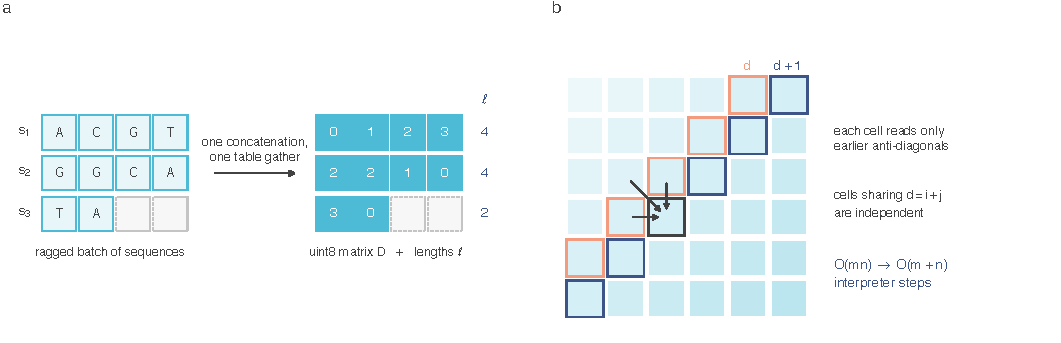
\includegraphics[width=\textwidth]{figures/fig1_design.pdf}
\caption{\textbf{Seqcore's array representation and the wavefront recurrence.}
\textbf{a}, A ragged batch of sequences is stored as one padded matrix $D$ of
ordinals together with a vector $\ell$ of true lengths. Encoding is a single
table gather over the concatenated batch, so its cost does not scale with the
number of sequences. Dotted cells are padding, excluded by the length mask.
\textbf{b}, In the alignment matrix, each cell reads only cells on earlier
anti-diagonals, so all cells sharing $d = i+j$ are mutually independent and are
evaluated in one vector operation. This reduces interpreter-level iteration from
$O(mn)$ to $O(m+n)$ without altering the recurrence.}
\label{fig:design}
\end{figure}

\section{Results}
\label{sec:results}

\subsection{Benchmarking procedure}

Measurements were taken on two machines: \BenchHost{} running
\BenchPlatform, and \OtherMachine{} with \OtherCores{} vCPUs. Both run CPython
\BenchPython, NumPy \BenchNumpy{} and Biopython \BenchBiopython{} so that
hardware is the only difference between them; unless stated otherwise, reported
numbers are from the \PrimaryMachine, and Section~\ref{sec:res:platform}
compares the two. We include a desktop-class Apple silicon machine because it is
increasingly the hardware on which this kind of analysis is actually run. Each
configuration runs in a
freshly spawned subprocess, so import order, allocator state and warmed caches
cannot leak between implementations, and each reported time is the best of five
repetitions (three for alignment and $k$-mer counting) --- the appropriate
statistic for throughput on a machine that is not otherwise quiesced. Sequences
are uniformly random over $\{A,C,G,T\}$ from a fixed seed.

The pure-Python comparison uses the fastest obvious standard-library formulation
of each operation (for instance \texttt{str.count} for GC content and
\texttt{str.translate} for reverse complement), not a deliberately naive one. It
is included because it is a meaningful baseline: for several operations it
outperforms Biopython, and a library that cannot beat it is not earning its
dependency.

The benchmark driver (\texttt{benchmarks/benchmark\_suite.py}) and its raw JSON
output are committed to the repository, and every figure and
Table~\ref{tab:summary} is regenerated from that output by
\texttt{paper/make\_figures.py}. No number in this manuscript is transcribed by
hand.

\begin{figure}[t]
\centering
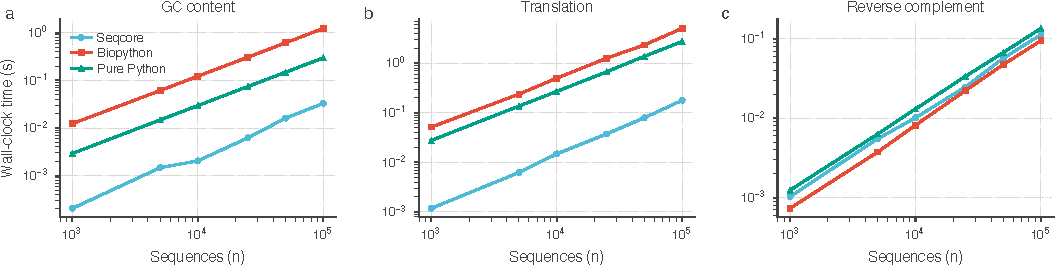
\includegraphics[width=\textwidth]{figures/fig2_batch.pdf}
\caption{\textbf{Scaling of batch operations} on sequences of $\BatchLen$\,bp,
measured on the \PrimaryMachine, shown log--log. All implementations are linear in batch size; what differs is the
constant factor. \textbf{a}, GC content. \textbf{b}, Translation. \textbf{c},
Reverse complement, where a single compiled pass
(\texttt{str.translate} in Biopython) is already close to the memory-bandwidth
limit and Seqcore obtains no advantage.}
\label{fig:batch}
\end{figure}

\subsection{Batch operations}

Figure~\ref{fig:batch} shows scaling up to $\BatchN$ sequences of
$\BatchLen$\,bp. All implementations are linear in batch size, as expected; the
separation is in the constant. At $\BatchN$ sequences Seqcore computes GC
content in $\GCms$\,ms and translates in $\TransMs$\,ms, corresponding to
single-core throughputs of $\GCthroughput$\,Gbase\,s$^{-1}$ and
$\TransThroughput$\,Mbase\,s$^{-1}$.

Translation shows the largest margin ($\TransVsBio\times$ Biopython,
$\TransVsPy\times$ pure Python) because it is the operation where the conventional approach pays the most
per residue: a Python-level dictionary lookup and a transient string per codon.
Replacing that with an integer index into a lookup table removes both costs at
once. GC content behaves similarly, though the absolute margin over pure Python
($\GCvsPy\times$) is smaller because \texttt{str.count} is itself a compiled scan.

\begin{figure}[t]
\centering
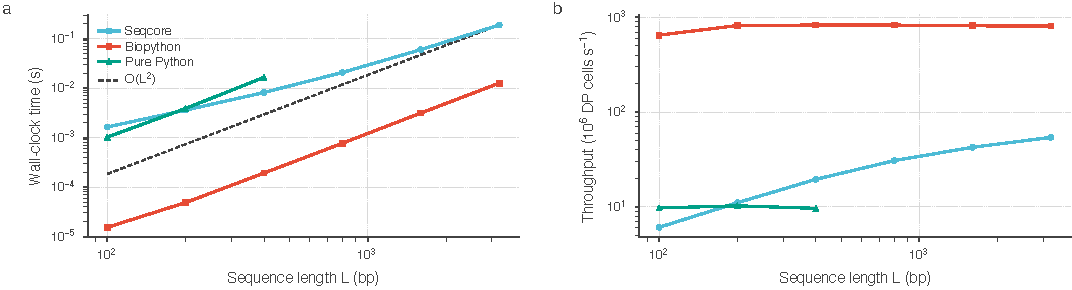
\includegraphics[width=\textwidth]{figures/fig3_alignment.pdf}
\caption{\textbf{Pairwise global alignment}, measured on the \PrimaryMachine.
\textbf{a}, Wall-clock time against sequence length. Seqcore converges to the
$O(L^2)$ reference slope at large $L$; at small $L$ it is dominated by fixed
per-call NumPy overhead. The scalar Python implementation is omitted above
400\,bp, where it becomes impractical.
\textbf{b}, The same data as dynamic-programming cell throughput. Seqcore's
throughput rises with $L$ as the fixed cost of each vector operation is
amortized over longer anti-diagonals, but plateaus well below Biopython's
compiled aligner.}
\label{fig:align}
\end{figure}

\subsection{Pairwise alignment}

Figure~\ref{fig:align} shows alignment cost against sequence length. Seqcore's
cell throughput rises from $\AlignCellsLo$ to $\AlignCellsHi$ million
cells\,s$^{-1}$ as $L$ grows from $\AlignLenLo$ to $\AlignLenHi$\,bp, because the fixed cost of each vector operation is
amortized over progressively longer anti-diagonals; at small $L$ the diagonals
are short and per-call overhead dominates, which is why the curve in
Figure~\ref{fig:align}a is visibly sub-quadratic there before converging to the
$O(L^2)$ reference.

Biopython's aligner sustains roughly $\AlignBioCells$ million cells\,s$^{-1}$ across the
whole range --- flat, as expected for compiled code with no per-call interpreter
cost. Seqcore does not approach this and is not intended to;
Section~\ref{sec:limits} states the consequence for users.

\subsection{$k$-mer counting}
\label{sec:res:kmers}

Figure~\ref{fig:kmers}a shows the behaviour predicted in
Section~\ref{sec:kmers}. For $k \le 10$, where $4^k$ is at or below the window
count and $k$-mers collapse heavily, the integer path is $\KmerEightSpeedup\times$
faster than the string counter at $k=8$. Beyond the crossover nearly every window is
distinct, the integer path would lose, and the dispatch rule routes those cases
to \texttt{Counter}; measured times for $k \ge 12$ therefore reflect the fallback
and remain $\KmerTwelveSpeedup\times$ faster than pure Python through the batched
string handling alone. The empirical crossover falls at $k=\KmerCross$, exactly where $4^k$
first exceeds the number of windows.

\begin{figure}[t]
\centering
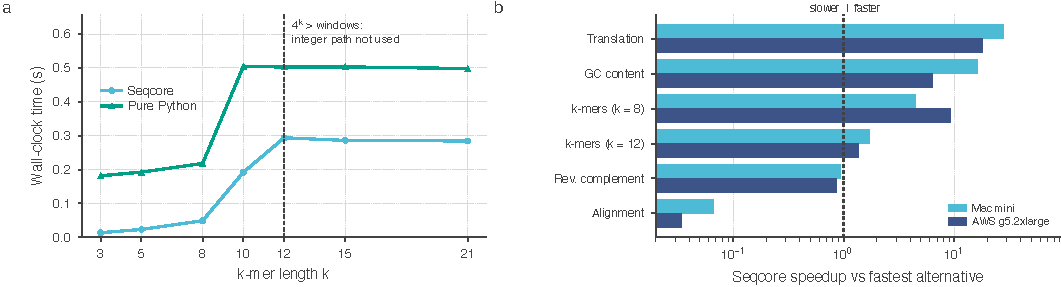
\includegraphics[width=\textwidth]{figures/fig4_kmers_summary.pdf}
\caption{\textbf{$k$-mer counting and cross-operation summary.}
\textbf{a}, $k$-mer counting for 2000 sequences of 1000\,bp. The integer-encoding
path wins while $k$-mers collapse; the dashed line marks the $4^k > N$ dispatch
rule, beyond which Seqcore falls back to a string counter rather than
regressing. Biopython provides no batch $k$-mer counter and is omitted.
\textbf{b}, Seqcore's speedup relative to the faster of Biopython and pure Python
for each operation, on both machines, at the configurations in
Table~\ref{tab:summary}. Bars left of the dashed line are operations where
Seqcore is slower. The ordering of operations is the same on both machines.}
\label{fig:kmers}
\end{figure}

\subsection{Behaviour across machines}
\label{sec:res:platform}

Absolute times depend strongly on the machine, so it is worth asking whether any
conclusion does. Figure~\ref{fig:kmers}b repeats the comparison on both
machines. Seqcore is $\PrimaryFasterLo$--$\PrimaryFasterHi\times$ faster on the
\PrimaryMachine{} than on the \OtherCPU{} in absolute terms, but the sign of
every comparison is identical: the same three operations win, the same two lose,
and the $k$-mer dispatch crossover falls at the same $k$.

The magnitudes do move, and in both directions. GC content is
$\GCvsBio\times$ Biopython on the \PrimaryMachine{} against
$\OtherGCvsBio\times$ on the \OtherCPU, because Apple silicon executes the
vectorized reduction proportionally faster than it executes Biopython's
per-object loop. $k$-mer counting goes the other way: its margin over pure
Python is \emph{larger} on the server, whose interpreter is comparatively slower
than its NumPy. The lesson is that a single-machine speedup figure should be
read as one point estimate, not a property of the library --- which is why we
report two machines and commit the harness that produced both.

\subsection{Where Seqcore is not the right tool}
\label{sec:limits}

Two operations do not favour this design, and we state them plainly rather than
omitting them.

\textbf{Reverse complement} runs at $\RCvsBio\times$ Biopython ($\RCms$\,ms versus
$\RCbioms$\,ms at $\BatchN$ sequences; $\OtherRCvsBio\times$ on the \OtherCPU). Biopython implements it as \texttt{str.translate}
followed by a slice: two compiled passes over contiguous bytes, with no padding
and no gather indirection. Seqcore performs comparable byte-level work on a
padded matrix, and the operation is memory-bandwidth bound rather than dispatch
bound, so removing interpreter overhead cannot help. There is no vectorization
advantage available here, and we do not claim one.

\textbf{Pairwise alignment} is roughly $\AlignSlower\times$ slower than Biopython's
aligner at $L=\AlignLenHi$ (and $\OtherAlignSlower\times$ slower on the
\OtherCPU). The wavefront still issues $O(m+n)$ NumPy calls, each materializing
temporaries proportional to the diagonal length, whereas Biopython dispatches
into compiled code with none of that overhead. Vectorized NumPy narrows the gap
against scalar Python but cannot close it against C; that requires a compiled
kernel. Users whose workload is alignment-bound should use a dedicated aligner,
and Seqcore's documentation says so at the call site.

Two further limitations are worth recording. Seqcore's \texttt{align()} accepts a
\texttt{gap\_extend} argument that currently has no effect: gaps are scored
linearly using \texttt{gap\_open} alone, and affine gap penalties are not yet
implemented. This is documented in the function's docstring and covered by a
regression test. Separately, Seqcore ships CuPy
device-management utilities, but no analysis kernel dispatches to the GPU; all
Seqcore results in this paper are single-core CPU measurements
(see Section~\ref{sec:res:gpu}).

\subsection{What a GPU backend could and could not deliver}
\label{sec:res:gpu}

Seqcore does not currently compute on the GPU. Because the representation in
Section~\ref{sec:layout} is a plain numeric array, porting the elementwise
kernels to CuPy~\cite{okuta2017cupy} is mechanically straightforward, so it is
worth measuring what that port would be worth before undertaking it. We
transcribed four Seqcore kernels to CuPy against the identical ordinal matrix,
verified that they reproduce the CPU results, and timed them on an NVIDIA A10G
(Figure~\ref{fig:gpu}). Timings synchronize the CUDA stream inside the measured
region, since CuPy launches kernels asynchronously.

The result is a caution against the obvious headline. Measured with the matrix
already resident on the device, the kernels are 23--326$\times$ faster than
Seqcore's CPU path. Measured per call from host memory --- which is what a user
calling \texttt{sc.reverse\_complement(arr)} would actually experience --- the
same kernels are 5--20$\times$ faster, because transferring the batch across
PCIe costs more than the arithmetic. For reverse complement, which performs one
table lookup per byte, transfer accounts for 97\% of the elapsed time; the
operation with the highest arithmetic intensity, $k$-mer counting at $k=8$,
retains almost all of its advantage.

Both numbers are correct measurements of different situations, and
Figure~\ref{fig:gpu}c shows the relationship between them: if the encoded matrix
stays on the device across $N$ successive operations, the single transfer is
amortized and the effective speedup rises from the per-call value towards the
resident-data limit. For reverse complement the crossover is fast --- three
chained operations already double the benefit --- whereas $k$-mer counting
begins near its ceiling.

The design implication is specific. A GPU backend implemented per function, with
each call copying in and out, would deliver roughly $5\times$ on the
bandwidth-bound operations. Capturing the larger factor requires
\texttt{DNAArray} itself to hold device memory, transferring only at the I/O
boundaries. That is an architectural decision about where the array lives, not a
kernel-level optimization, and it is the form the work will take.

We report no GPU performance for Seqcore itself, because there is none to
report; Figure~\ref{fig:gpu} characterizes a planned backend, not the shipping
library. The transfers use pageable host memory, so the per-call figures are a
conservative bound: pinned staging buffers would raise them somewhat without
changing the structure of the argument.

\begin{figure}[t]
\centering
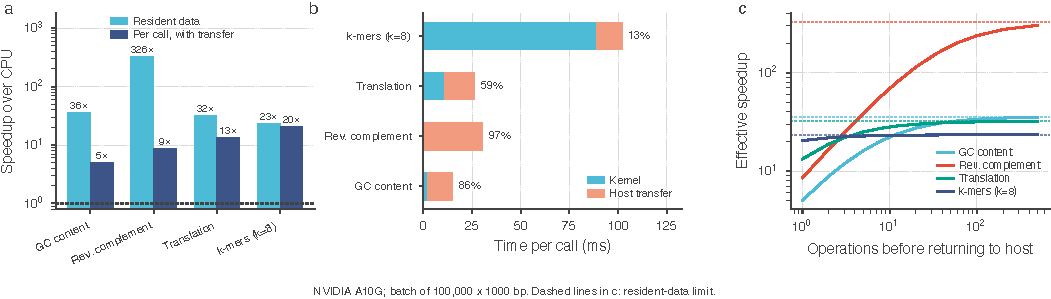
\includegraphics[width=\textwidth]{figures/fig5_gpu.pdf}
\caption{\textbf{What a GPU backend would be worth.} CuPy transcriptions of
Seqcore's kernels on an NVIDIA A10G, against Seqcore's CPU path on the same
host. \textbf{a}, Speedup measured with data already resident on the device
(light) and per call including host transfer (dark). \textbf{b}, Where the
per-call time goes; the annotation gives the transfer share. \textbf{c},
Effective speedup when $N$ operations are chained before returning results to
the host, so the transfer is paid once; dashed lines mark the resident-data
limit from panel~\textbf{a}. \emph{Seqcore does not currently use the GPU} ---
these are measurements of a prospective backend, not of the shipping library.}
\label{fig:gpu}
\end{figure}

\begin{table}[t]
\centering
\caption{\textbf{Summary of measured performance} on the \PrimaryMachine.
Times are best-of-$N$ wall clock in seconds. \emph{Speedup} is Seqcore relative to the faster of Biopython
and pure Python for that operation; values below $1.0$ indicate Seqcore is
slower. Biopython provides no batch $k$-mer counter. This table is generated from
the committed benchmark output by \texttt{paper/make\_figures.py} and shares its
source with Figure~\ref{fig:kmers}b.}
\label{tab:summary}
\setlength{\tabcolsep}{5pt}
\footnotesize
% Generated by paper/make_figures.py -- do not edit by hand.
\begin{tabular}{llrrrr}
\toprule
Operation & Configuration & Seqcore (s) & Biopython (s) & Pure Python (s) & Speedup \\
\midrule
GC content & $100{,}000 \times 1000$\,bp & 0.021 & 1.241 & 0.344 & $16.2\times$ \\
Translation & $100{,}000 \times 1000$\,bp & 0.078 & 3.895 & 2.180 & $27.9\times$ \\
Reverse complement & $100{,}000 \times 1000$\,bp & 0.099 & 0.093 & 0.119 & $0.94\times$ \\
Global alignment & $L=3200$\,bp & 0.189 & 0.013 & --- & $0.07\times$ \\
$k$-mers ($k=8$) & $2{,}000 \times 1000$\,bp & 0.049 & --- & 0.218 & $4.44\times$ \\
$k$-mers ($k=12$) & $2{,}000 \times 1000$\,bp & 0.294 & --- & 0.503 & $1.71\times$ \\
\bottomrule
\end{tabular}

\end{table}

\section{Discussion}

Seqcore's premise is that the representation, not the algorithm, is what usually
limits this class of Python library. None of the techniques used here are novel
in themselves --- masked reductions, lookup tables and wavefront dynamic
programming are all standard --- but they only become available once a batch of
sequences is a dense numeric array rather than a list of objects. Choosing that
representation first is what makes the rest follow.

Two points generalize beyond this library. The first is that an optimization
needs a stated domain of applicability. The $k$-mer result is the clearest case:
the same integer encoding is a large win at small $k$ and a regression at large
$k$, and only the $4^k \le N$ dispatch rule makes it safe to enable by default.
Reporting the mean speedup over a favourable set of $k$ would have hidden this
entirely.

The second is that a benchmark is only meaningful if a reader can rerun it. The
comparisons here are generated by a committed script whose raw output is also
committed, and the figures and table in this paper are produced from that output
mechanically. We would encourage this as a default for software papers: it costs
little, and it makes the difference between a performance claim and a
reproducible measurement.

Finally, we think reporting the unfavourable comparisons is part of the
contribution rather than a caveat to it. A library that is $\GCvsBio\times$ faster
than Biopython at GC content and $\AlignSlower\times$ slower at pairwise alignment is
useful, but only to a user who can tell which regime they are in. Presenting only
the favourable half would make the library harder to use correctly, not easier.

\subsection*{Future work}

The clearest remaining gap is alignment, which needs a compiled kernel rather
than further NumPy refinement. The GPU backend analysed in
Section~\ref{sec:res:gpu} is the other main direction, and the measurement there
sets its design: it must keep the encoded matrix resident on the device rather
than transferring per call. The harness used for that analysis
(\texttt{benchmarks/benchmark\_gpu.py}) is included in the repository so the
same question can be re-asked on other hardware.

\section*{Availability and requirements}

\noindent
\textbf{Project name:} Seqcore \\
\textbf{Project home page:} \url{https://github.com/pritampanda15/Seqcore} \\
\textbf{Operating systems:} Platform independent (tested on Linux, macOS, Windows) \\
\textbf{Programming language:} Python $\ge 3.9$ \\
\textbf{Other requirements:} NumPy $\ge 1.22$; optional Biopython, pandas, h5py,
RDKit, MDAnalysis, CuPy \\
\textbf{Licence:} MIT \\
\textbf{Version described here:} \SeqcoreVersion{} \\
\textbf{Installation:} \texttt{pip install seqcore>=\SeqcoreVersion}

\noindent
Everything reported here is reproduced from the repository root with:

\begin{lstlisting}[language=bash]
pytest                                   # correctness and equivalence suite
python benchmarks/benchmark_suite.py     # Figures 2-4, Table 1
python paper/make_figures.py             # regenerate figures and table
\end{lstlisting}

\section*{Competing interests}
The author declares no competing interests.

\section*{Data availability}
All benchmark inputs are synthetic and generated from fixed random seeds by the
committed benchmark script. Raw timing output is committed under
\texttt{benchmarks/results/}.

\begin{thebibliography}{9}
\small

\bibitem{cock2009biopython}
Cock PJA, Antao T, Chang JT, \emph{et al.}
Biopython: freely available Python tools for computational molecular biology and
bioinformatics.
\emph{Bioinformatics} 25(11):1422--1423, 2009.

\bibitem{harris2020numpy}
Harris CR, Millman KJ, van der Walt SJ, \emph{et al.}
Array programming with NumPy.
\emph{Nature} 585:357--362, 2020.

\bibitem{needleman1970}
Needleman SB, Wunsch CD.
A general method applicable to the search for similarities in the amino acid
sequence of two proteins.
\emph{Journal of Molecular Biology} 48(3):443--453, 1970.

\bibitem{smith1981}
Smith TF, Waterman MS.
Identification of common molecular subsequences.
\emph{Journal of Molecular Biology} 147(1):195--197, 1981.

\bibitem{wozniak1997}
Wozniak A.
Using video-oriented instructions to speed up sequence comparison.
\emph{Bioinformatics} 13(2):145--150, 1997.

\bibitem{rognes2011}
Rognes T.
Faster Smith-Waterman database searches with inter-sequence SIMD
parallelisation.
\emph{BMC Bioinformatics} 12:221, 2011.

\bibitem{okuta2017cupy}
Okuta R, Unno Y, Nishino D, Hido S, Loomis C.
CuPy: A NumPy-compatible library for NVIDIA GPU calculations.
\emph{Proceedings of the Workshop on Machine Learning Systems (LearningSys) at
NIPS}, 2017.

\end{thebibliography}

\end{document}
